\documentclass{article}

\usepackage{pgf}
\usepackage{tikz}
\usetikzlibrary{arrows,automata}
\usepackage[latin1]{inputenc}
\begin{document}

	$q_{1}$: \texttt{ABCDHIJKMN}
	
	$q_{2}$: \texttt{BCDEGHIJKLMN}
	
	$q_{3}$: \texttt{BCDFGHIJKMN}
	
	\vspace{24pt}
	
	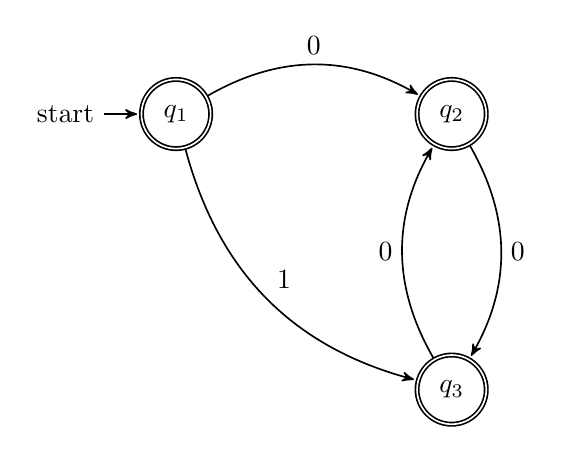
\begin{tikzpicture}[->,>=stealth',shorten >=1pt,auto,node distance=3.5cm,
	semithick]
	\tikzstyle{every state}=[fill=none,draw=#1,text=black]
	
	\node[initial,state,accepting] (A)                    {$q_{1}$};
	\node[state,accepting]          (B) [right of=A] {$q_{2}$};
	\node[state,accepting]          (C) [below of=B] {$q_{3}$};
	
	\path (A) edge [bend left]      node {0} (B)
	         (A) edge [bend right]   node {1} (C)
	         
	          (B) edge [bend left]     node {0} (C)
	          (C) edge [bend left]  node {0} (B);
	
	\end{tikzpicture}
	
\end{document}